\section{Introduction}
\label{sec:intro}

\begin{figure*}[t]
\centering
\IfFileExists{figures/fig1_comem_autofigure.pdf}
  {
\includegraphics[width=0.96\textwidth]{figures/fig1_comem_autofigure.pdf}}
  {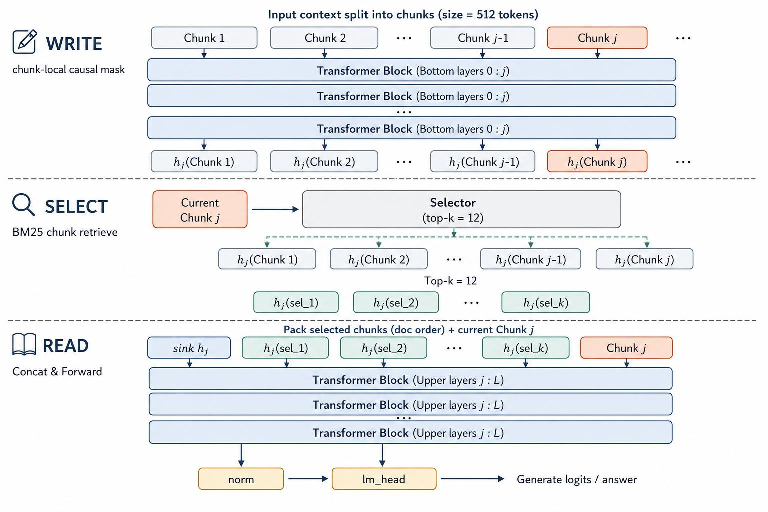
\includegraphics[width=0.96\textwidth]{figures/Structure.pdf}}
\caption{\textbf{CoMem treats transformer depth as a cross-query reuse axis.}
\textsc{Write} stores one intermediate residual per token, \textsc{Select}
retrieves a fixed working set, and \textsc{Read} resumes the upper layers with
the query present. The matched $j{=}0$ path retrieves the same chunks, order,
sink, and mask as raw text but recomputes every layer. The reported
$1.403\times$ is this matched depth effect; larger dense-to-bounded speedups
also include selection. A small left-overlap is evaluated as a focused repair
for missing lower-layer document context.}
\label{fig:teaser}
\end{figure*}

Repeated-query long-context serving can save work in two different ways.
Raw-text retrieval bounds the online token set but recomputes all layers
~\citep{rag,xu2024retrievallong}. Prefix, position-independent caching (PIC),
and modular-cache systems instead reuse precomputed document state, usually
layer-wise KV, while repairing position or context dependencies
~\citep{cacheblend,turborag,epic,cachecraft,kvpacket}. This paper asks a
narrower question: \emph{how much transformer depth should a reusable document
object prepay?}

\paragraph{Workload contract.}
We assume an open-weight model, a shared or slowly changing corpus, and enough
queries per document to amortize a model-version-specific Write. One-off
queries, frequently edited text, or corpora whose persistent states cannot be
kept near the accelerator may favor raw text. Every latency claim below names
whether it includes selection, state fetch, Write, model Read, and decode.

We instantiate that question with \textbf{CoMem} (Figure~\ref{fig:teaser}).
\textsc{Write} runs each context chunk through layers $[0{:}j)$ and stores one
residual vector per token. \textsc{Select} chooses a fixed number of chunks.
\textsc{Read} packs their residuals with the query and executes only
$[j{:}L)$ with full cross-pack attention. The endpoint $j{=}0$ stores token IDs
and replays the same selected pack through every layer. Thus $j$ varies prepaid
depth while holding evidence fixed.

Our strongest evidence is this \emph{matched $j{=}0\!\rightarrow\!12$
operating-point comparison}. On
Qwen3-8B, $j{=}12$ lowers isolated selected-pack Read from 931.9 to 664.4\,ms
($1.403\times$) but lowers a paired 15-cell RULER macro from 99.19 to 96.07.
This is not quality-preserving acceleration. A self-distilled upper-layer LoRA
is necessary to make the residual interface usable, and the 8\,KiB/token store
is worthwhile only when reused: CPU-pinned break-even ranges from 8.9--10.9
queries at 32k for generations up to 128 tokens, while the full GPU/CPU grid
ranges from 5.5--10.9. At 128k we retain only the one-generated-token points,
25.8--27.6 queries by store placement. Much larger dense-context numbers combine bounded
selection with depth reuse and are secondary operating points, not the causal
depth result.

We also test whether saved lower-layer compute can buy enough extra evidence to
offset the residual-interface loss. The answer is selector-dependent, but never
a CoMem aggregate win in our nine-cell diagnostic mixture. At matched online
latency, iterative-BM25 raw replay (maximum budget 10 chunks) beats CoMem
(budget 12) 64.78 to 53.22; frozen-BGE replay at budget 10 is 54.22 versus
53.22, with a dependence-aware hierarchical interval that crosses zero.
Selectors may under-fill these maximum budgets.
Thus this experiment bounds deployment conclusions rather than establishes a
new quality ranking over RAG or reusable-KV systems.

We also bound one source of error rather than claiming a complete explanation.
On a paired 8k/16k multikey diagnostic, document-contextual lower-layer states
close the 92.5-to-100.0 gap, while document-origin position remapping alone
reduces accuracy to 88.0. A deployable 32-token left overlap reaches 98.5 with
unchanged persistent bytes and per-query Read work. Because this repair is not
evaluated on the full natural-task suite, we treat it as a localized diagnosis
and engineering hypothesis.

\paragraph{Contributions.}
\begin{itemize}[leftmargin=1.2em,itemsep=1pt,topsep=2pt]
\item \textbf{Matched depth endpoint:} a same-evidence, same-adapter measurement of
the incremental benefit and quality cost of reusing lower-layer computation.
\item \textbf{Transparent system boundary:} persistent bytes, Write
amortization, serving crossover, and selector-dependent equal-latency results, with
bounded selection kept separate from depth reuse.
\item \textbf{Bounded diagnosis:} controlled continuous-state, context,
position, and overlap variants that isolate a major Write-side failure on one
paired multikey cohort without generalizing it beyond the evidence.
\end{itemize}
